\documentclass[english,twoside, openright, hidelinks, 11 pt, class=report,crop=false]{standalone}
\input{../../preamb}



\begin{document}
{\Large Eksamen Matematikk R1 våren 2025\hfill \\ {\footnotesize Løsning fra \color{blue} \href{https://sindreheggen.wordpress.com/}{OpenMathBooks prosjektet}}}	

\subsection*{Oppgave 1}
\[ f'(x)=x^4-2e^{-2x} \]

\subsection*{Oppgave 2}
\abc{
\item Da $e^x\neq 0$ for alle $x$, er $g(x)=0$ når $2x-1=0$, altså når $x=\frac{1}{2}$.
\item Vi setter $u=e^x$ og $v=(2x-1)^2=4x^2-4x+1$. Da er $u'=e^x$ og $v'=8x-4=4(2x-1)$. Av produktregelen ved derivasjon har vi at
\begin{align}
	g'(x)=\left(\frac{1}{2}uv\right)'&=\frac{1}{2}\left(u'v+uv'\right)\\
	&=\frac{1}{2}e^x(v+v')\\
	&=\frac{1}{2}e^x\left(4x^2-4x+1+4(2x-1)\right) \\
	&=\frac{1}{2}e^x\left(4x^2-4x-3\right)
\end{align}
Ved å gange ut parantesene kan vi bekrefte at $(2x+1)(2x-3)=4x^2-4x-3$, og dermed har vi vist det vi skulle.
\item Vi lager et fortegnsskjema for $g'(x)$. Da $\frac{1}{2}e^x>0$, er det bare de to andre faktorene som bidrar til at fortegnet forandrer seg.
\begin{figure}
	\centering
	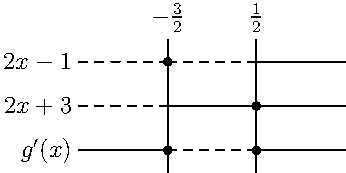
\includegraphics{opg2del1}
\end{figure}
At $g'(x)$ skifter fra positivt til negativt fortegn i $x=-\frac{3}{2}$, betyr at dette er et maksimalpunkt for $g$. Tilsvarende er $x=\frac{1}{2}$ et minimumspunkt for $g$. Videre er 
\begin{align*}
 g\left(-\frac{3}{2}\right) &= \frac{1}{2}e^{-\frac{3}{2}}\left(2\cdot\left(-\frac{3}{2}\right)-1\right)^2=2e^{-\frac{3}{2}}\vn
 g\left(\frac{1}{2}\right)&=\frac{1}{2}e^{\frac{1}{2}}\left(2\cdot\frac{1}{2}-1\right)^2=0
\end{align*}
$g$ har altså toppunkt $\left(-\frac{3}{2}, 2e^{-\frac{3}{2}}\right)$ og bunnpunkt $\left(\frac{1}{2}, 0\right)$
}

\subsection*{Oppgave 3}
\abc{
\item 
\begin{align*}
	content...
\end{align*}
}

\end{document} 